\textbf{R:} Comenzemos por recordar la impureza de Gini 

\[G(X_k) = \sum_{y \in X_k} p(y)(1-p(y))\]

Con lo que procedemos a calcular la probabilidad correspondiente a cada clase

\begin{align*}
    p(Y=0) = \frac{2}{4}=0.5\quad &\quad p(Y=1) = \frac{2}{4}=0.5
\end{align*}

Veamos ahora la impureza de Gini para la raíz:
\begin{align*}
    G(r) &= p(0)(1-p(0))+p(1)(1-p(1))\\
    &= 0.5(1-0.5)+0.5(1-0.5)\\
    &= 0.5
\end{align*}
Ahora, para formar el árbol debemos de ver un dato para realizar una partición, dado que todos los datos tienen el mismo valor para la característica Animal entonces se descarta y continuamos analizando a Doméstico, en este caso las primeras tres muestras indica un valor de $1$ mientras que la última indica un valor de $0$, con lo que se tiene la siguiente
\begin{center}
    \begin{tabular}{c|c|c}
    $\text{Doméstico}\geq 1$ & Verdadero & Falso \\
    \hline
    $Y$ & $\{1,0,1\}$ & $\{0\}$ \\
    \hline
    $p(Y=0)$ & $\frac{1}{3}$ & $1$ \\[0.1cm]
    $p(Y=1)$ & $\frac{2}{3}$ & $0$ \\[0.1cm]
    \hline
    $G$ & $\frac{1}{3}\cdot\frac{2}{3}+\frac{2}{3}\cdot\frac{1}{3}=\frac{4}{9}$ & $1\cdot(1-1)+0\cdot(1-0)=0$
    \end{tabular}
\end{center}

Ahora calcularemos la ganancia de información, esto se logra con las fórmulas

\begin{align*}
    IG(X,\phi) &= G(r)-E[G(X|\phi)]\\
    E[G(X|\phi)] &= \sum_{\phi} p(\phi) G(X|\phi)\\
\end{align*}

Entonces tenemos
\begin{align*}
    E[G(X|Domestico)] &= p(Domestico\geq 1) G(Domestico=1) \\&+ p(Domestico<1) G(Domestico=0)\\
    &= \frac{3}{4}\cdot\frac{4}{9}+\frac{1}{4}\cdot 0\\
    &= \frac{1}{3}\\
    IG(X, Domestico) &= G(r)-E[G(X|Domestico)]\\
    &= \frac{1}{2} - \frac{1}{3} = \frac{1}{6}
\end{align*}

Ahora veamos que ocurre con la característica Pequeño, en este caso las primeras dos muestras indican un valor de $0$ mientras que las últimas dos indican un valor de $1$, con lo que se tiene la siguiente

\begin{center}
    \begin{tabular}{c|c|c}
    $\text{Pequeño}\geq 1$ & Verdadero & Falso \\
    \hline
    $Y$ & $\{0,1\}$ & $\{1,0\}$ \\
    \hline
    $p(Y=0)$ & $\frac{1}{2}$ & $\frac{1}{2}$ \\[0.1cm]
    $p(Y=1)$ & $\frac{1}{2}$ & $\frac{1}{2}$ \\[0.1cm]
    \hline
    $G$ & $\frac{1}{2}\cdot\frac{1}{2}+\frac{1}{2}\cdot\frac{1}{2}=\frac{1}{2}$ & $\frac{1}{2}\cdot\frac{1}{2}+\frac{1}{2}\cdot\frac{1}{2}=\frac{1}{2}$
    \end{tabular}
\end{center}

Calculamos ahora la ganancia de información para esta característica
\begin{align*}
    E[G(X|Peque\text{ñ}o)] &= p(Peque\text{ñ}o\geq 1) G(Peque\text{ñ}o=1) \\&+ p(Peque\text{ñ}o<1) G(Peque\text{ñ}o=0)\\
    &= \frac{1}{2}\cdot\frac{1}{2}+\frac{1}{2}\cdot\frac{1}{2}\\
    &= \frac{1}{2}\\
    IG(X, Peque\text{ñ}o) &= G(r)-E[G(X|Peque\text{ñ}o)]\\
    &= \frac{1}{2} - \frac{1}{2} = 0
\end{align*}

Ahora que tenemos ambas ganancias, podemos concluir que la característica que se debe de elegir para realizar la partición es Doméstico quien será el nodo raíz.\\
Para la siguiente partición, notemos que la rama  $Domestico\geq 1? = falso$ es pura, por lo que no se puede seguir dividiendo, ahora para la rama $Domestico\geq 1? = verdadero$ veremos que sucede con la característica Pequeño, tomamos las primeras tres muestras y veamos que

\begin{center}
    \begin{tabular}{c|c|c}
    $\text{Pequeño}\geq 1$ & Verdadero & Falso \\
    \hline
    $Y$ & $\{0, 1\}$ & $\{1\}$ \\
    \hline
    $p(Y=0)$ & $\frac{1}{2}$ & $1$ \\[0.1cm]
    $p(Y=1)$ & $\frac{1}{2}$ & $0$ \\[0.1cm]
    \hline
    $G$  
    & $ \frac{1}{2}\cdot(1-\frac{1}{2}) + \frac{1}{2}\cdot(1-\frac{1}{2})=\frac{1}{2} $
    & $ 1\cdot(1-1) + 0\cdot(1-0)=0 $
    \end{tabular}
\end{center}
Notemos que en el caso don de $Peque\text{ñ}o\geq 1? = falso$ de $G$ de $0$ lo cual indica que es una rama pura. Por lo que se tiene la siguiente ganancia de información
\begin{align*}
    E[G(X|Peque\text{ñ}o)] &= p(Peque\text{ñ}o\geq 1) G(Peque\text{ñ}o=1) \\&+ p(Peque\text{ñ}o<1) G(Peque\text{ñ}o=0)\\
    &= \frac{2}{3} \cdot \frac{1}{2} + \frac{1}{3} \cdot 0\\
    &= \frac{1}{3}\\
    IG(X, Peque\text{ñ}o) &= G(Domestico\geq 1)-E[G(X|Peque\text{ñ}o)]\\
    &= \frac{4}{9} - \frac{1}{3} = \frac{1}{9}
\end{align*}

Se construye el siguiente árbol de desición
\begin{center}
    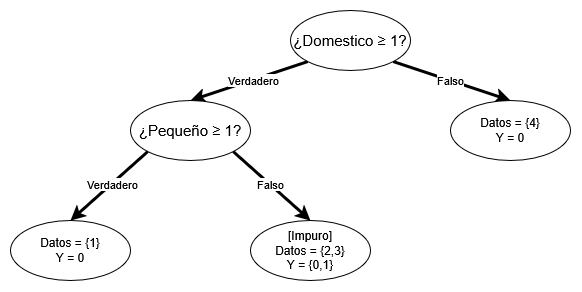
\includegraphics[height = 8cm]{ejercicios/assets/ej3_arbol.png}
\end{center}

Veamos que $IG > 0$ de Pequeño por lo que se intenta dividir por medio de esta característica, la rama $Peque\text{ñ}o\geq 1? = verdadero$ es impura ya que $G= \frac{1}{2}$ y dado que no quedan más características para realizar divisiones, el algoritmo se detiene con una hoja impura por lo que no se logra terminar en hojas en cada clase.